\section{System Architecture}
Figure \ref{fig:system} contains the intended architecture of DSNAT, and how various components relate to it.

\begin{figure}[htbp]
  \centering
    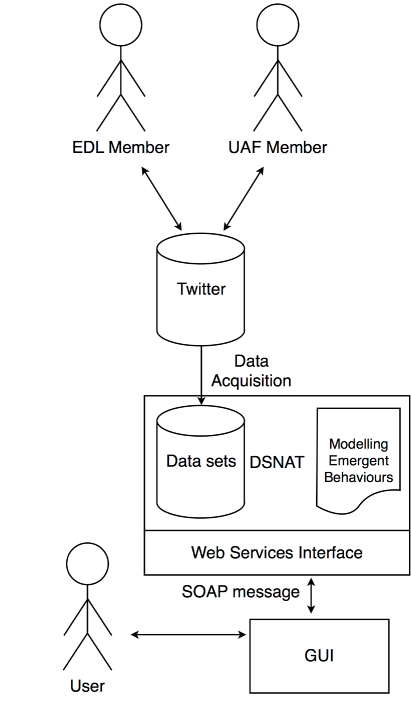
\includegraphics[width=0.4\textwidth]{./img/system}
  \caption{DSNAT system architecture.}
  \label{fig:system}
\end{figure}

The GUI component of the system is being reused from the social network analysis tool \cite{snat} created in the previous year, and what changes will need to me made to adapt it for use with our tool are described in more detail in Section \ref{sec:des_gui}.

We will be collecting data from Twitter from users relating the English Defence League and Unite Against Fascism, amongst other available datasets. The data we acquire will be processed and included into a selection of datasets, from which the tool will then be able to perform various algorithms for analysis.

A portion of this project is research based in the direction of ``Modelling Emergent Behaviours''. With the completion of DSNAT we are hoping to apply the results of this research on much large networks than currently used.

DSNAT forms the core component of the project. Within DSNAT we aiming to have a Hadoop cluster implemented, upon which algorithms for analysing social networks and influence propagation within networks can be executed. The datasets collected during the data acquisition phase of the project will be stored within DSNAT, for processing by users. DSNAT itself will be presented via a web services interface, so that users can remotely connect to DSNAT.